\chapter{\positron\electron pair background as the largest background contribution}
\label{PairBkg}

\begin{chapterabstract}
 At the International Linear Collider, the collision of the two lepton beams goes hand in hand with the production of background particles.
 Unlike at hadron colliders, the main background contribution does not arise from QCD processes and underlying events, but rather from the interaction of the colliding beam's electromagnetic fields.
 The created secondary \positron\electron pairs form a significant background, the so-called pair background, for the inner detectors, and therefore need to be studied in great detail.
 This chapter discusses the effect of the ILC beam parameters on the pair background, and the impact of the \positron\electron pairs on the \sid detector.
\end{chapterabstract}

As discussed in Section~\ref{BeamBeam}, the pair background is a high cross section process from beam-beam interactions and the main source of background at the ILC.
The secondary electrons and positrons show a characteristic density distribution, which reach to the inner layers of the \sid vertex and tracking detectors.
The impact on the \sid detector is studied with respect to the timing, the hit distribution, and the arising detector occupancy.
These impacts are, however, affected by the change in the ILC beam parameters for the ILC250 stage, which is another study done for this thesis and is explained throughout the following sections.
The results of these studies contributed towards design choices of the accelerator and the \sid detector.

\section{The background generator GuineaPig}
\label{PairBkg:GuineaPig}
For studying the effects of the pair background, \positron\electron pairs from beam-beam interactions were generated with the Monte Carlo (MC) background event generator \guineapig~\cite{Schulte:1997nga} version 1.4.4. 
When providing the accelerator beam parameters, the pair background events of one bunch crossing are simulated and stored in an ASCII output file named ``pairs.dat''.
The parameters used for generating the pair background for this thesis are given in Appendix~\ref{Appendix:Pairs:GuineaPig}. 
\\Since the ASCII files cannot directly serve as input to a full \geant~\cite{geant_ref,geant_ref2} detector simulation, a conversion tool was written in context of this thesis, and instructions on its usage are available in~\cite{Confluence}. 
The tool converts the ASCII output to one of the following common file formats: stdhep or slcio~\cite{LCIO}.
These file formats are directly applicable with the \geant based simulation tool \slic~\cite{Graf:2006ei}, which simulates interactions of the input particles with matter.
The geometry of the simulated world is described in a lcdd file in a human-readable format.
The flexible geometry description allows the simulation of particle interactions with individual detector geometries.
To this end, the geometry description file ``sidloi3'' of the \sid detector, which was used for the simulation studies in this and in the following chapters, is based on the detector design described in Section~\ref{ILC:SiD} and in~\cite[p. 69 ff]{TDR4}.

\section{Pair background envelopes}
\label{PairBkg:helix}
Analyzing the generated pair background events, it becomes apparent that the \positron\electron pairs have a low transverse momentum.
Figure~\ref{fig:PairBkg:Momentum} shows the distribution of their longitudinal and transverse momentum for the two ILC stages at \SI{250}{\GeV} and \SI{250}{\GeV} center-of-mass energy.
\todo{Describe the momentum distributions}
 \begin{figure}[h]
 \centering
  \begin{subfigure}[b]{0.49\textwidth}
   \centering
    \includegraphics[width=\textwidth]{placeholder.jpg}
   \caption{Longitudinal momentum}
   \end{subfigure}
   \hfill
    \begin{subfigure}[b]{0.49\textwidth}
   \centering
    \includegraphics[width=\textwidth]{placeholder.jpg}
   \caption{Transverse momentum}
   \end{subfigure}
   \caption[Pair background momentum distributions]{Comparison of the pair background momentum distributions for the ILC at \SI{250}{\GeV} and \SI{250}{\GeV} center-of-mass energy, with the longitudinal momentum shown in Figure (a) and the transverse momentum in Figure (b).}
   \label{fig:PairBkg:Momentum}
 \end{figure}
\\Due to their low transverse momentum, the pairs are deflected on helical tracks in the magnetic field of the detector solenoid magnet.
An algorithm was written that calculates the helix tracks of the pair particles using their four-vectors.
The track positions are computed from the radius of the helix, its center position and its pitch. The following assumptions were made for the algorithm:
The magnetic field in the proximity of the IP is homogeneous, with a field strength of \SI{5}{\tesla} for the SiD solenoid.
The particle momenta do not change in the region of interest for this analysis, because of which the helix radius is constant.
Any particle interaction with other particles or with matter is not taken into account.
\\Figure~\ref{fig:helix_circle} shows schematically the projection of a helix onto the xy-plane.
Depending on the particle's charge the orientation of the helix is determined.
\begin{figure}
    \centering
    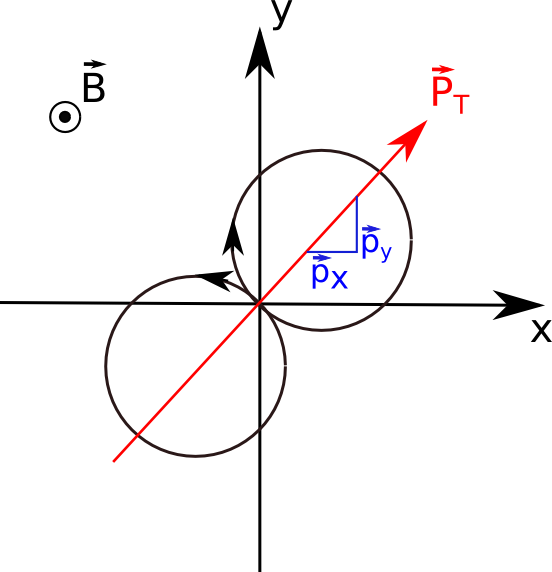
\includegraphics[width=0.3\textwidth]{Figures/Pairs/Helix_explanation.png}
    \caption[Schematic projection of the helix on the xy-plane]{
    This schematic shows the projection of a helix track onto the xy-plane, with the vector of the transverse momentum (P\textsubscript{T}) and the the x- and y-momenta (p\textsubscript{x} and p\textsubscript{y}).
    Depending on the particle's charge, the direction of the rotation is either clockwise or anticlockwise.
    The center, the radius, and the orientation of the projected circle is dependent on the transverse momentum of the particle.
    }
    \label{fig:helix_circle}
\end{figure}
The pair density is then plotted using the helix track algorithm to calculate the position in x and y for a given position in z.
For the ILC stage at \SI{500}{\GeV}, the pair background was generated with \guineapig, and its density plotted in Figure~\ref{fig:PairBkg:Density} (a).
The envelope of all the tracks shows a characteristic bell shape, with the highest density along the z axis.
Since the bell shaped distribution is fully symmetrical in positive and negative z-direction as well as in the xz and yz-plane, the chosen view of the pair background envelopes will in the following always be of the xz-plane in positive z-direction.
\\In order to compare the envelope shapes for different ILC beam parameters, Figure~\ref{fig:PairBkg:Density} (b) only shows the envelope outlines containing a certain fraction of all tracks.
In this way, it becomes apparent that for higher center-of-mass energies the width of the envelope increases.
At \SI{500}{\GeV}, the envelope containing \SI{99.99}{\percent} of all pair helix tracks crosses the beam pipe, extending towards the innermost layer of the SiD vertex detector, which has a radius of \SI{14}{\milli\meter}.
For lower center-of-mass energies, the envelopes stay within the beam pipe radius.
The pair background simulation files for this comparison plot were generated with \guineapig as well, using the beam parameters of the three different baseline ILC stages~\cite[p. 11]{TDR1}.
 \begin{figure}[h]
 \centering
  \begin{subfigure}[b]{0.49\textwidth}
   \centering
    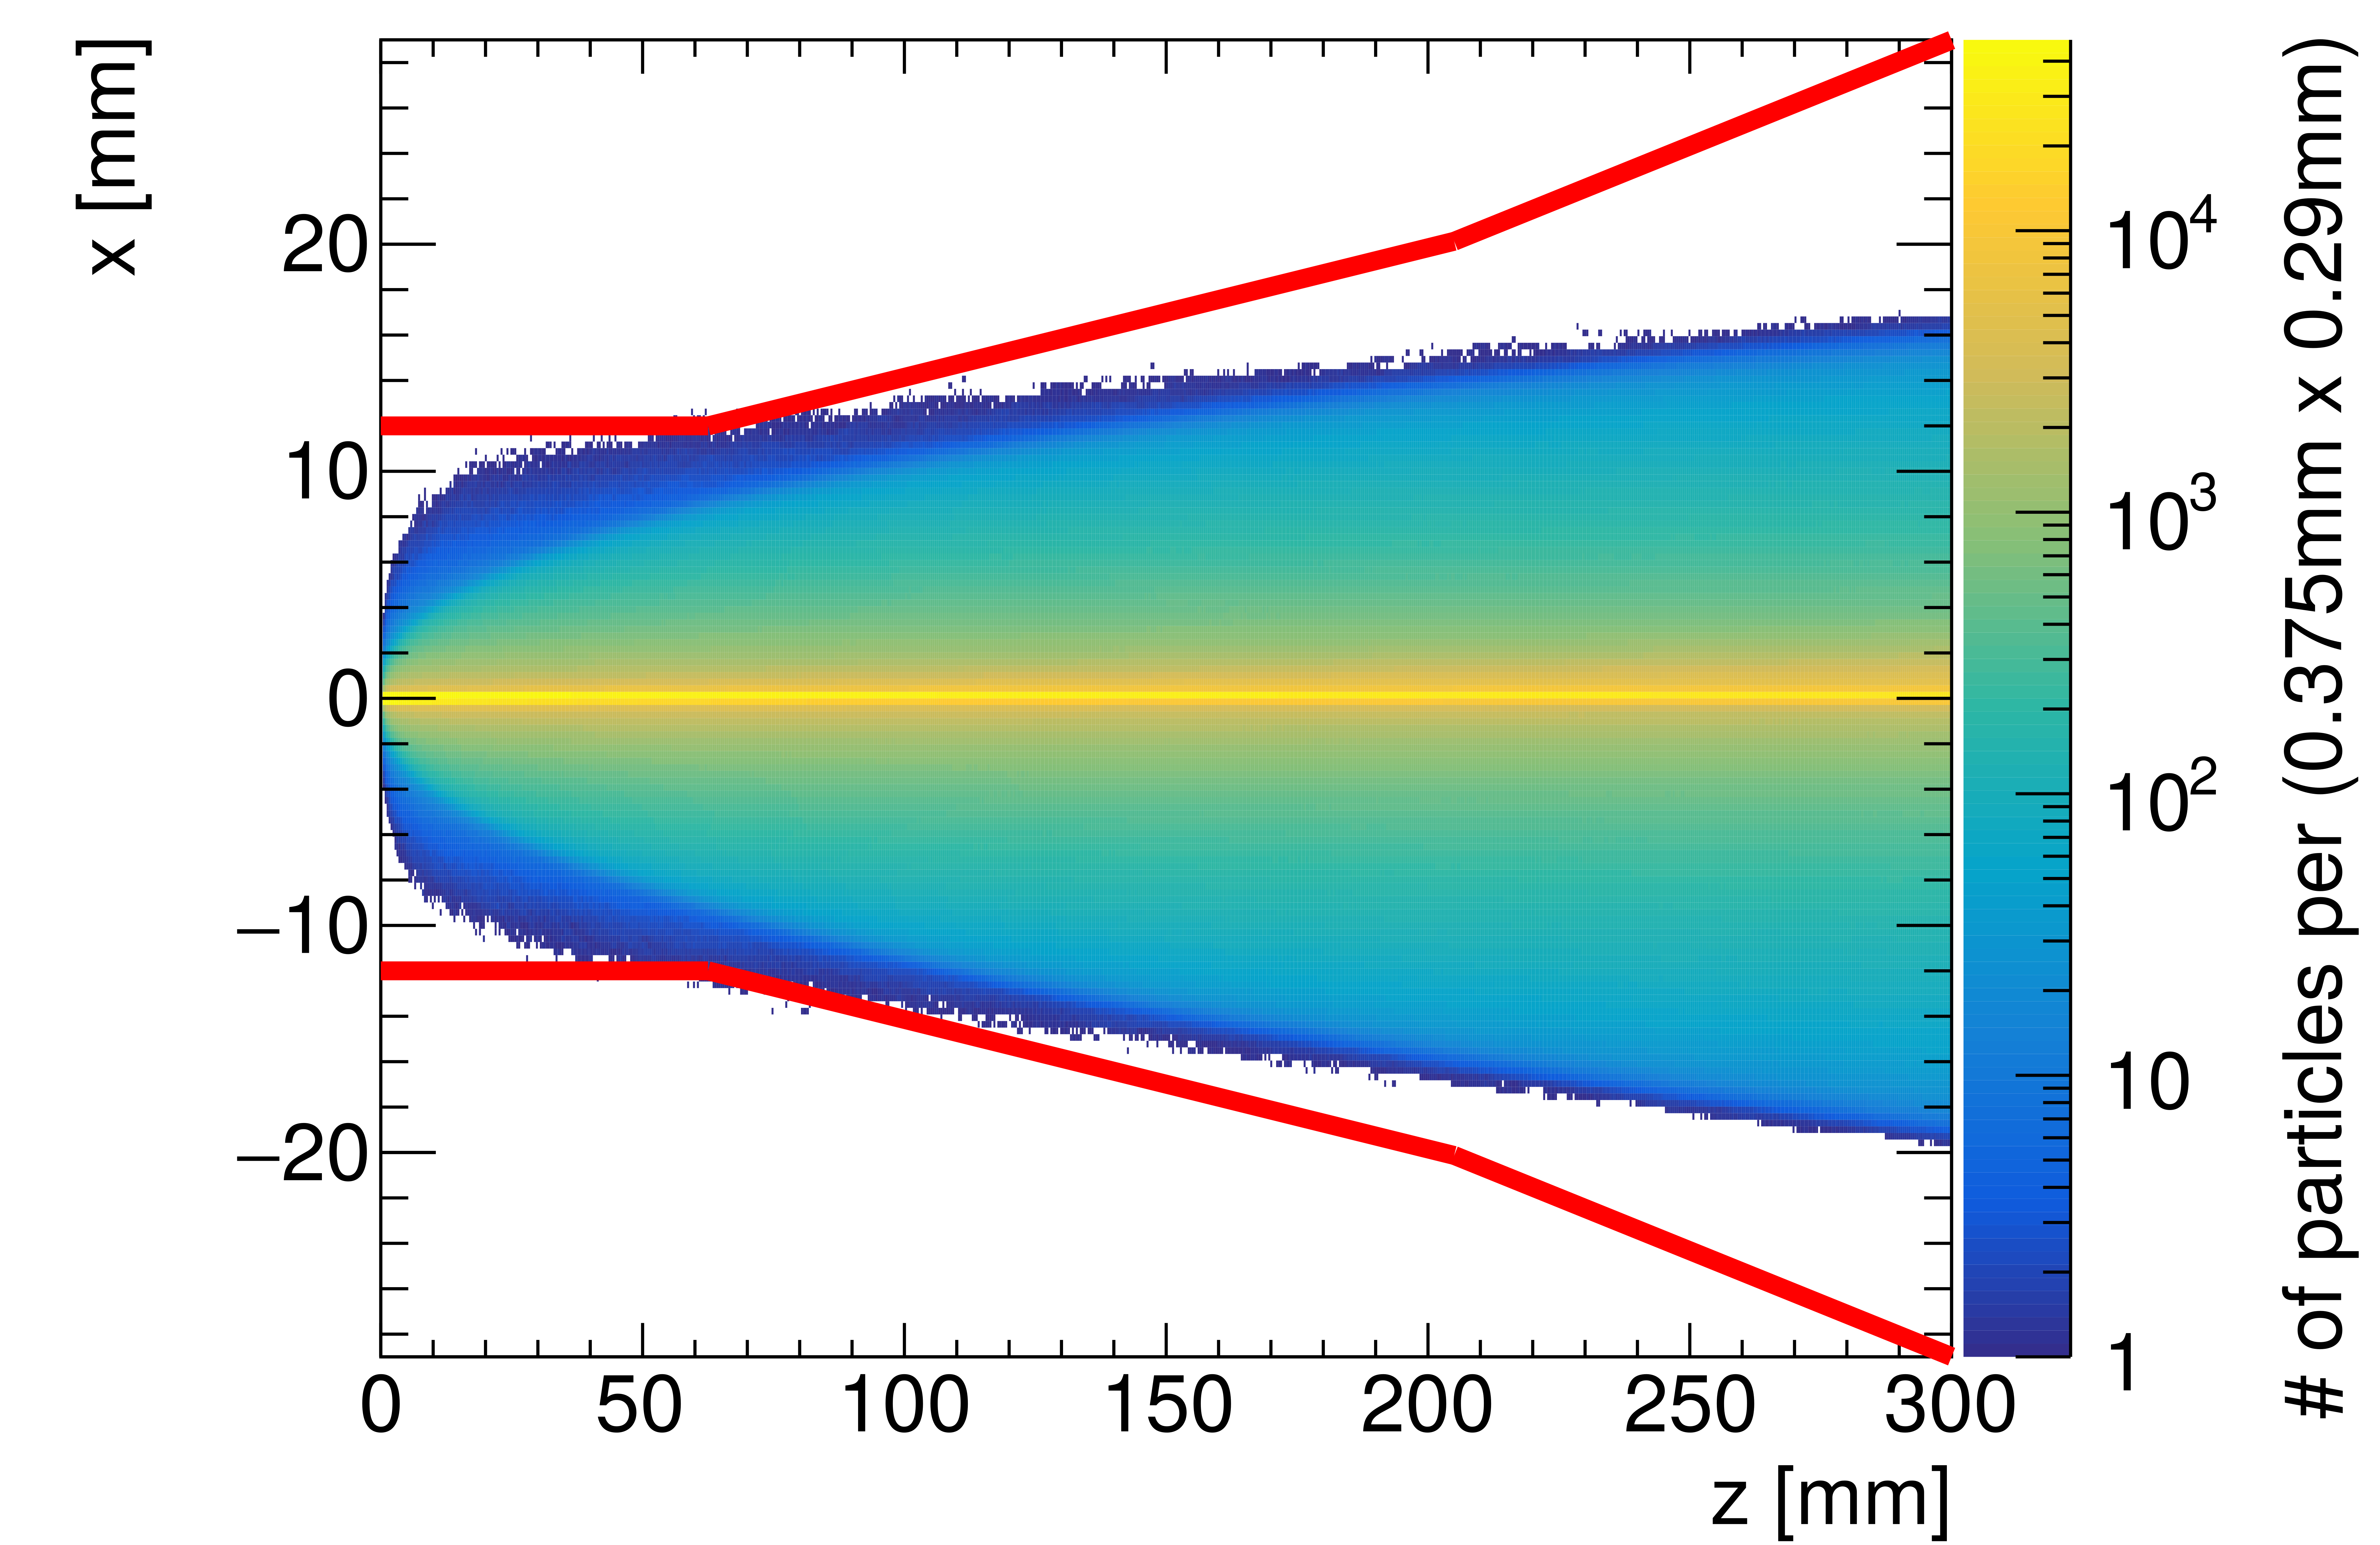
\includegraphics[width=\textwidth]{Figures/Pairs/Helix_tracks_xz_80bunches_500GeV_5T.png}
   \caption{Pair backgound density for the ILC500}
   \end{subfigure}
   \hfill
    \begin{subfigure}[b]{0.49\textwidth}
   \centering
    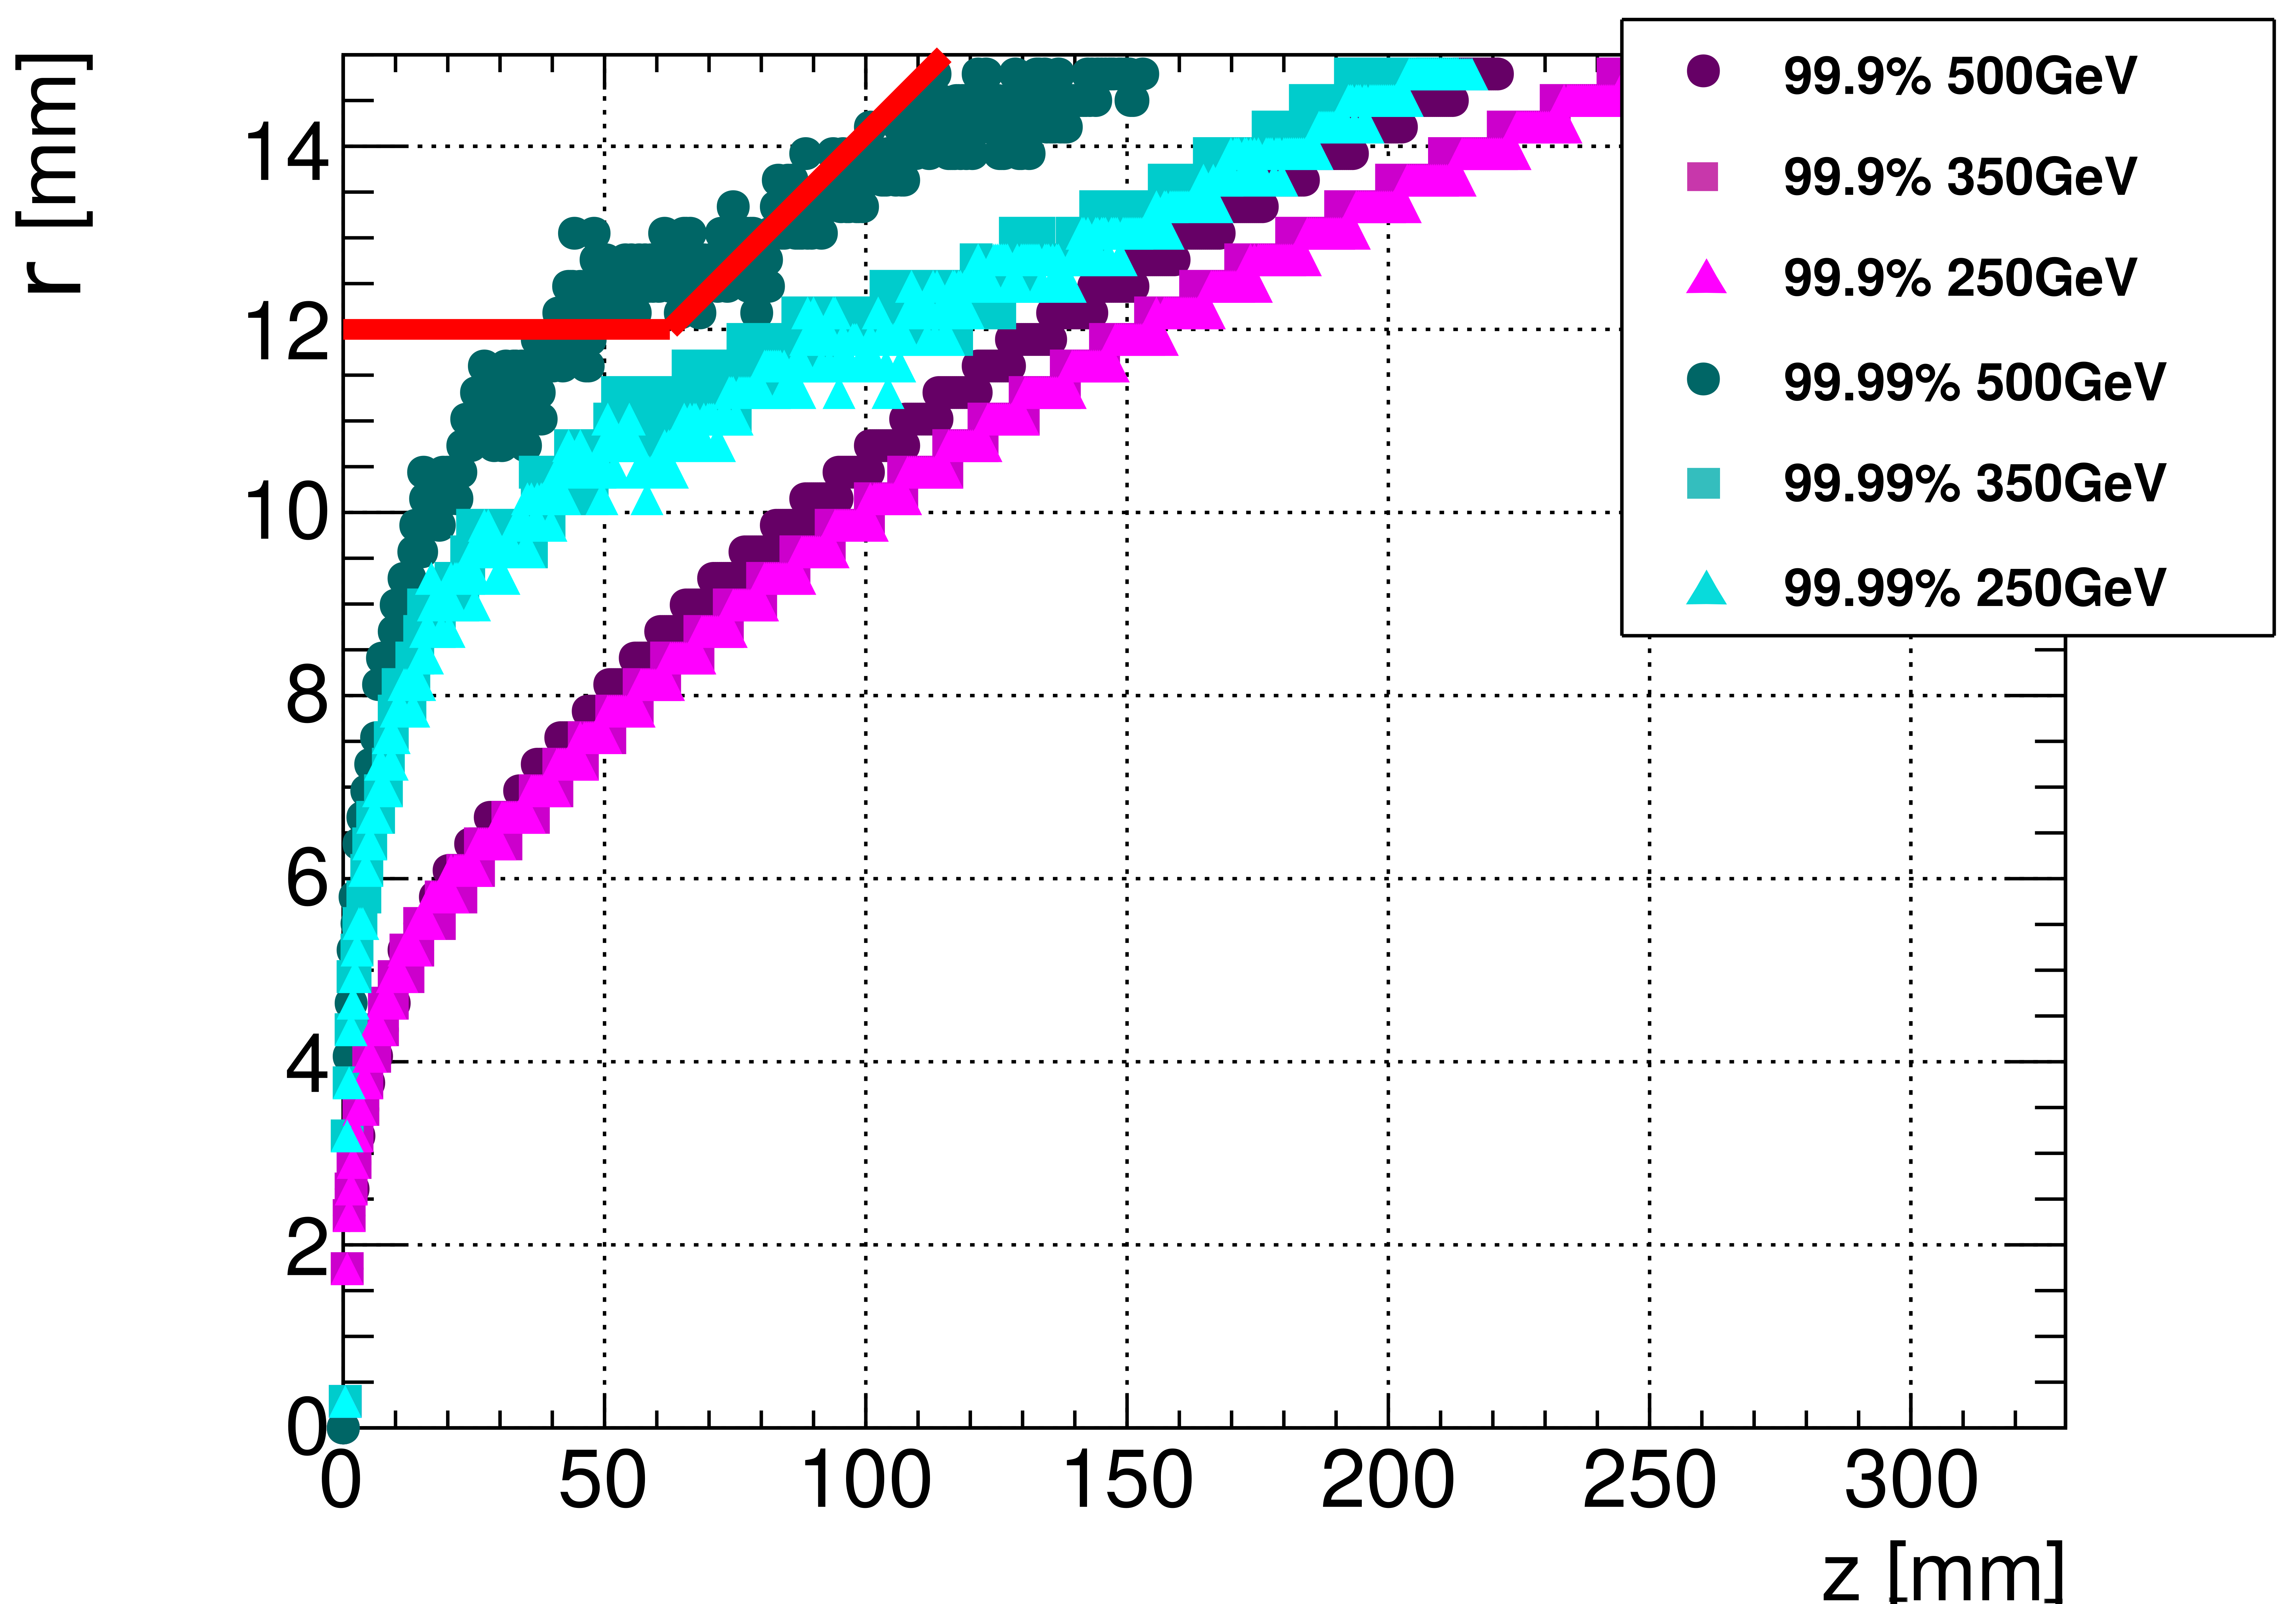
\includegraphics[width=\textwidth]{Figures/Pairs/HelixEnvelopes_COMPARISON_xz_500_350_250_comparison_EDITED_2.png}
   \caption{yz-plane}
   \end{subfigure}
   \caption[Pair background density]{The figures display the pair background density in the xz-plane for one ILC bunch crossing.
   Figure (a) shows the complete track density distribution of the pairs at the ILC stage at a center-of-mass energy of \SI[detect-all]{500}{\GeV}.
   The color scale shows the number of tracks per unit area.
   The red solid lines represent the outline of the beam pipe
   \\In Figure (b), the density envelopes of three ILC stages are compared: at 250, 350, and \SI[detect-all]{500}{\GeV}.
   For that purpose, not the complete density distribitution is plotted, but rather the envelope outlines containing either \SI[detect-all]{99.9}{\percent} or \SI[detect-all]{99.99}{\percent} of all tracks.
   }
   \label{fig:PairBkg:Density}
 \end{figure}
 
As explained in Section~\ref{ILC:layout:staging}, the first ILC stage will be at \SI{250}{\GeV} instead of the originally anticipated \SI{500}{\GeV}.
Due to this decision in 2017, efforts have been made to study a possible change in the baseline beam parameters for this stage in order to increase the luminosity from \num{8.2} to \SI{16.2e34}{\per\centi\meter\squared\per\second}~\cite{LCWS17_paper}. 
To this end, three alternative beam parameter sets have been suggested, which vary from the original baseline parameters in the emittance and the beta function values.
The values which differ are listed in Table~\ref{tab:ILC250_sets}.
For all alternative sets, the horizontal emittance $\epsilon_x$ is reduced. 
Additionally, the horizontal and vertical beta functions at the IP, $\beta^*_x$ and $\beta^*_y$, are changed for sets (B) and (C).
Since both, the emittance and the beta function, are dependencies of the beam size, they enter indirectly the Equation~\ref{eq:luminosity} for the beam luminosity.
\\On the other hand however, a reduced horizontal emittance implies also an increase in the beam-beam interactions and in the pair background level.
For the process of deciding the new official beam parameter set, a study of the impact of this increased pair background on the \sid vertex detector performance was therefore a crucial step.
In the following, the simulation studies of the pair background for the four parameter schemes listed in Table~\ref{tab:ILC250_sets} are presented.
\begin{table}[h]
\caption[New ILC250 beam parameters]{Changes between the baseline and alternative beam parameter sets for the ILC stage at \SI[detect-all]{250}{\GeV}~\cite{LCWS17_paper}.
The highlighted parameter set (A) was chosen to be the new official scheme for the ILC250.}
\label{tab:ILC250_sets}
\centering
\begin{tabularx}{0.42\textwidth}{c|ccc}
\hline\hline
\textbf{Set} & $\epsilon_x$ (\si{\micro\meter}) & $\beta^*_x$ (\si{\milli\meter}) & $\beta^*_y$ (\si{\milli\meter})\\
\hline
 Baseline & 10.0 & 13.0 & 0.41\\
\rowcolor{Gray} (A) & 5.0 & 13.0 & 0.41\\
 (B) & 5.0 & 9.19 & 0.41\\
 (C) & 5.0 & 9.19 & 0.58\\
\hline\hline
\end{tabularx}
\end{table}




\section{Occupancy studies and buffer depth}
\label{PairBkg:occupancy}
Definition of occupancy and dead cells already in BDS muon chapter!
\begin{itemize}
 \item sidloi3
 \item Occupancy studies for ILC250 parameter sets compared with ILC500 TDR
 \item Occupancy studies for ILC250 parameter sets for different SiD designs (old L*, w/o antiDiD etc) - insert plots
 \item Occupancy studies for ILC250 parameter sets in dependency of phi and z - insert plots
\end{itemize}

\subsection{Hit maps of the SiD subdetectors}
\label{PairBkg:hitmaps}
\todo{Show with projection of hitmaps that there are more hits on edges of VertexBarrel detector (because of helix envelopes)}
%TODO TH1D* histo=Layer_1->ProjectionX("ProjectionX",1,Layer_1->GetNbinsY(),"e")


\section{Hit time distributions}
\label{PairBkg:hittime}

\begin{itemize}
 \item Time distribitution of pairs - redo for ILC250
 \item Plots of particle origins - redo for ILC250
 \item Possible reduction of background through time gates
\end{itemize}

